% =====================================================================
%  Part: the five extra experiments (fisherfaces_experiments.m).
%  Included from study_guide.tex.
% =====================================================================

\part{Five experiments beyond the paper}
\label{part:experiments}

\texttt{fisherfaces\_simple.m} answers \emph{does it work}. This part answers
five harder questions, each one implemented in
\texttt{fisherfaces\_experiments.m} and each producing a figure. Every number
quoted here comes from \texttt{run\_log\_experiments.txt}.

Two of the five are things the paper itself does not do (E3, E4), one is a
check that nobody usually runs (E2), one is the paper's \emph{actual} protocol
which our headline table skips (E5), and one measures the quantity that decides
whether the whole method is numerically safe (E1).

%% =====================================================================
\section{E1: how badly conditioned is \texorpdfstring{$\Sw$}{S\_W} as
\texorpdfstring{$m$}{m} grows?}
\label{sec:e1}

\paragraph{The question.} The paper sets $m = N-c$. At exactly that value $\Sw$
has rank $m$: full rank, but with \textbf{zero slack} --- one more PCA direction
and it would be singular. ``Nearly singular'' is vague, so measure it.

\paragraph{The maths.} For a symmetric positive definite matrix,
\[
  \kappa(\Sw) \;=\; \frac{\lambda_{\max}(\Sw)}{\lambda_{\min}(\Sw)} ,
\]
and the rule of thumb is that about $\log_{10}\kappa$ of the $16$ significant
decimal digits double precision gives us are lost when solving with $\Sw$.

$m$ is squeezed from \emph{both} sides:
\[
  \boxed{\;c-1 \;\le\; m \;\le\; N-c\;}
\]
The upper bound keeps $\Sw$ invertible (Theorem~\ref{thm:rankSw}). The lower
bound is easy to forget: we extract $c-1$ directions, and a space of dimension
$m$ cannot supply more than $m$ of them. On ORL the whole window is
$31 \le m \le 160$. We found this bound the hard way --- the first version of
the sweep started at $m=20$ and crashed asking for $31$ Fisherfaces out of a
$20$-dimensional space.

\paragraph{The result.}

\begin{center}
\small
\begin{tabular}{rrrr@{\hskip 2em}rrrr}
\toprule
\multicolumn{4}{c}{\textbf{ORL} ($N=192$, $c=32$)} &
\multicolumn{4}{c}{\textbf{Yale} ($N=1520$, $c=38$)} \\
$m$ & $\rank(\Sw)$ & $\kappa(\Sw)$ & rate &
$m$ & $\rank(\Sw)$ & $\kappa(\Sw)$ & rate \\
\midrule
 31 &  31 & $6.49\times10^{1}$ & 94.5 &  100 &  100 & $3.62\times10^{3}$ & 51.6 \\
 40 &  40 & $7.73\times10^{1}$ & 93.0 &  200 &  200 & $1.20\times10^{4}$ & 56.3 \\
 60 &  60 & $1.75\times10^{2}$ & \textbf{95.3} &  400 &  400 & $4.91\times10^{4}$ & 65.2 \\
 80 &  80 & $3.73\times10^{2}$ & 91.4 &  700 &  700 & $2.42\times10^{5}$ & 68.8 \\
100 & 100 & $6.40\times10^{2}$ & 91.4 & 1000 & 1000 & $1.10\times10^{6}$ & \textbf{69.8} \\
120 & 120 & $1.69\times10^{3}$ & 90.6 & 1200 & 1200 & $3.64\times10^{6}$ & 69.4 \\
140 & 140 & $5.80\times10^{3}$ & 89.1 & 1400 & 1400 & $4.17\times10^{7}$ & 66.8 \\
150 & 150 & $2.22\times10^{4}$ & 91.4 & 1450 & 1450 & $4.26\times10^{8}$ & 68.0 \\
155 & 155 & $2.38\times10^{5}$ & 89.8 &      &      &                    &      \\
160 & 160 & $7.85\times10^{7}$ & 90.6 & 1482 & \textbf{1481} & $6.01\times10^{12}$ & 67.2 \\
\bottomrule
\end{tabular}
\end{center}

\begin{figure}[htbp]
\centering
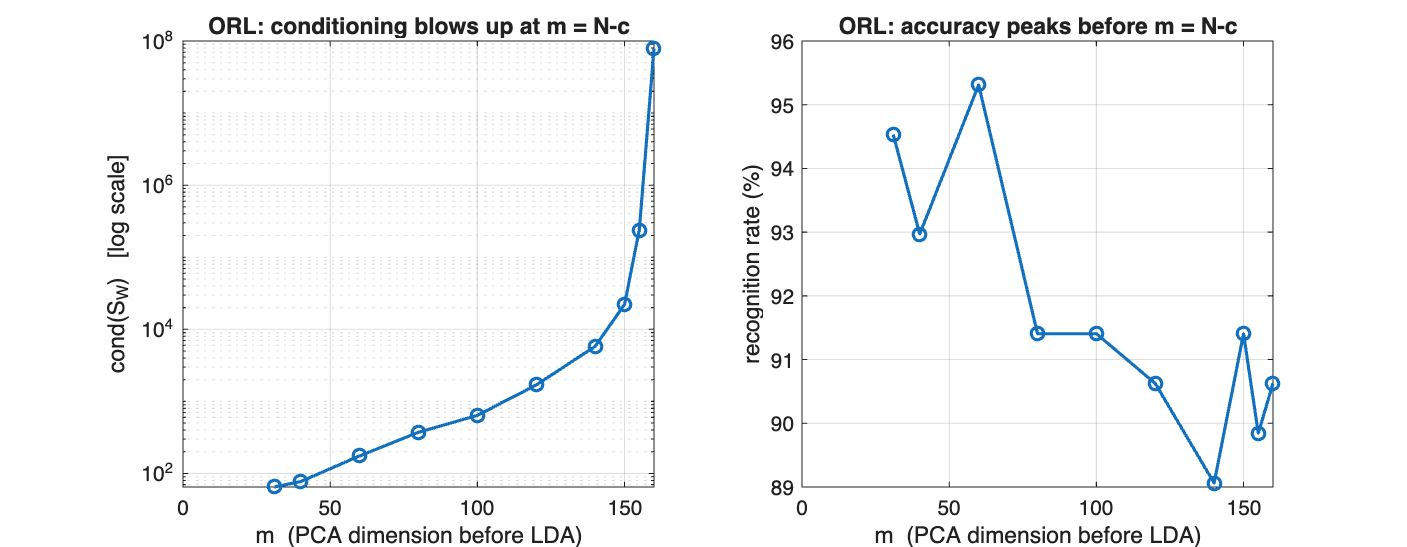
\includegraphics[width=\textwidth]{figs_experiments/E1_cond_vs_m_ORL.png}
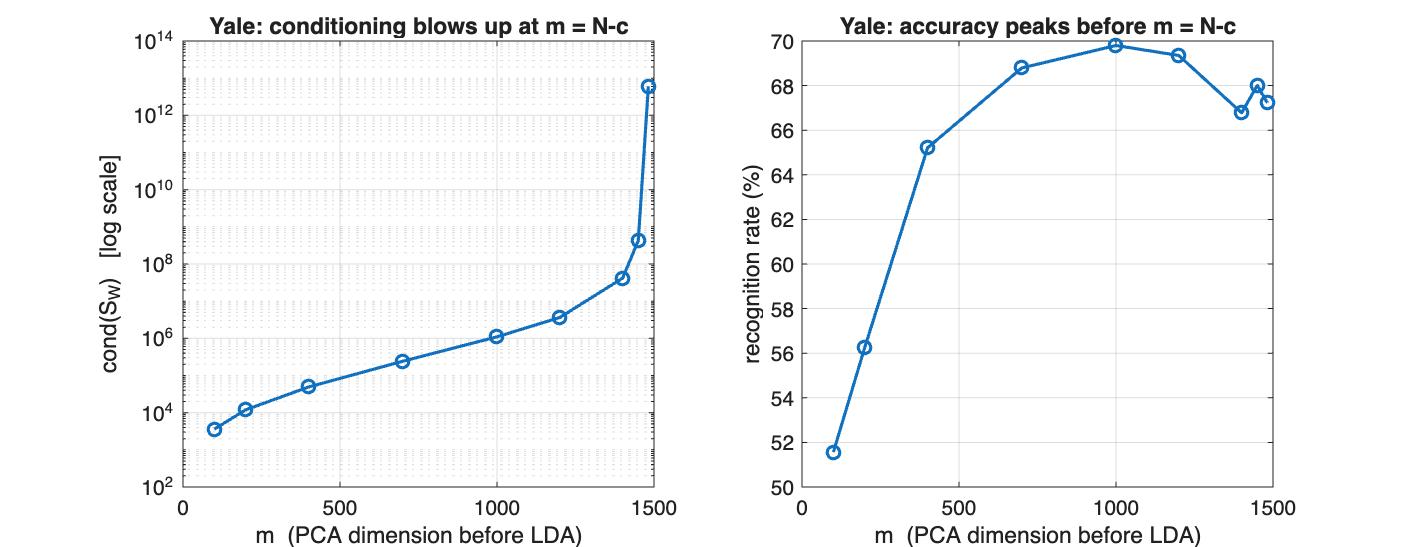
\includegraphics[width=\textwidth]{figs_experiments/E1_cond_vs_m_Yale.png}
\caption{Condition number (log scale) and recognition rate against $m$. The
conditioning is flat for most of the range and then turns almost vertical in
the last few steps before $m = N-c$, while accuracy has already peaked and
started falling.}
\end{figure}

\begin{observation}[Three things worth saying out loud]
\emph{First, the growth is not gradual.} On ORL $\kappa$ rises by a factor of
$1.2\times10^{6}$ across the sweep, but most of that happens in the last three
points: $5.8\times10^{3}$ at $m=140$ becomes $7.85\times10^{7}$ at $m=160$. On
Yale the total factor is $1.66\times10^{9}$, and the last step alone
($1450 \to 1482$) multiplies $\kappa$ by $14000$.

\emph{Second, the paper's choice is not the best choice on either database.}
ORL peaks at $m=60$ with $95.3\%$ against $90.6\%$ at $m=N-c$; Yale peaks at
$m=1000$ with $69.8\%$ against $67.2\%$. Accuracy turns down well before
conditioning becomes alarming, so this is not purely a numerical effect: the
extra directions are fitting noise.

\emph{Third, at Yale's $m = N - c$ the matrix is not even nominally full rank.}
\texttt{rank} returns $1481$, not $1482$ --- see the gotcha in
Section~\ref{sec:rankcholgotcha}.
\end{observation}

\subsection{Does the naive solver survive this sweep?}
\label{sec:naivesweep}

Section~\ref{sec:naive} argued that $\Sw^{-1}\Sb$ is fine \emph{on our data}
despite having no guarantees. E1 is the natural place to stress that claim,
because it visits the worst-conditioned matrices in the project. Running both
routes at every $m$:

\begin{center}
\small
\begin{tabular}{lrrrrr}
\toprule
 & $\kappa(\Sw)$ & rate (Cholesky) & rate (naive) & $\max|\operatorname{Im}\lambda|$ & subspace angle \\
\midrule
ORL,  $m=31$   & $6.5\times10^{1}$  & 94.5 & 94.5 & $0$                  & $0.00^\circ$ \\
ORL,  $m=160$  & $7.8\times10^{7}$  & 90.6 & 90.6 & $9.3\times10^{-10}$  & $0.00^\circ$ \\
Yale, $m=1000$ & $1.1\times10^{6}$  & 69.8 & 69.8 & $1.0\times10^{-13}$  & $0.00^\circ$ \\
Yale, $m=1482$ & $6.0\times10^{12}$ & 67.2 & 67.2 & $2.3\times10^{-7}$   & $0.00^\circ$ \\
\bottomrule
\end{tabular}
\end{center}

Identical at every $m$ on both databases. But notice what \emph{is} moving:
$\max|\operatorname{Im}\lambda|$ climbs from $0$ to $2.3\times10^{-7}$, a factor
of about $100$ between Yale's $m=1400$ and $m=1482$ alone. The round-off is
growing exactly as the conditioning predicts --- it simply has not yet grown
enough to change a nearest-neighbour decision. The margin is shrinking and
there is no guarantee, only a measurement.

\begin{gotcha}[``$\Sw$ is full rank so the naive route is fine'' is the wrong defence]
\label{sec:rankcholgotcha}
It is tempting to justify the naive route by saying PCA has made $\Sw$ full
rank. Two problems. First, it is not PCA that is full rank --- the PCA basis has
rank $N-1$ whatever we do --- it is $\Sw$ \emph{in the reduced space}, and only
when $m \le N-c$. Second, at Yale's $m = 1482$ MATLAB's \texttt{rank} reports
\textbf{1481}, so by that test $\Sw$ is \emph{not} full rank, and both routes
work anyway.

Both answers are correct, because they use different tolerances.
\texttt{rank}'s default is
$\max(\text{size})\cdot\varepsilon\cdot\lambda_{\max}
= 1482 \cdot 2.22\times10^{-16}\lambda_{\max} = 3.3\times10^{-13}\lambda_{\max}$,
while the smallest eigenvalue sits at $1.7\times10^{-13}\lambda_{\max}$: below
\texttt{rank}'s threshold, above what Cholesky needs.

So do not argue from full rank. Argue from the measurement: \emph{\texttt{chol}
succeeds, so $\Sw$ is positive definite to working precision, and both routes
agree to $0.00^\circ$ at every $m$ we tested.} Full rank makes the naive route
\emph{defined}; it does not make it \emph{accurate}, which is a separate axis.
\end{gotcha}

%% =====================================================================
\section{E2: is the result real, or is the pipeline leaking?}

\paragraph{The question.} We report $90.6\%$. How do we know that number comes
from faces, rather than from a bug that lets training information reach the
test set?

\paragraph{The maths.} Shuffle the \emph{training} labels at random and change
nothing else. Now there is no relationship between a face and its label, so no
method can beat guessing, which is
\[
  \text{chance} \;=\; \frac{100}{c} \;=\; \frac{100}{32} \;=\; 3.1\% .
\]
Any method still scoring well after this was never using the faces.

\begin{lstlisting}
shuffle  = randperm(oN);
ytrShuf  = oYtr(shuffle);
\end{lstlisting}

\paragraph{The result.}

\begin{center}
\begin{tabular}{lcc}
\toprule
 & true labels & shuffled labels \\
\midrule
eigenfaces ($k=c-1$) & $94.5\%$ & $0.8\%$ \\
Fisherfaces          & $90.6\%$ & $0.0\%$ \\
chance ($100/c$)     & \multicolumn{2}{c}{$3.1\%$} \\
\bottomrule
\end{tabular}
\end{center}

\begin{figure}[htbp]
\centering
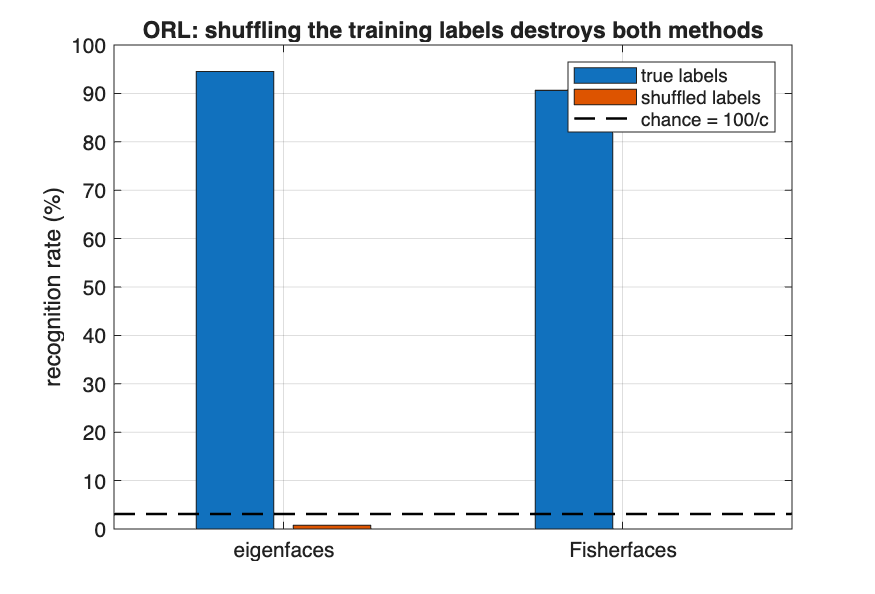
\includegraphics[width=0.62\textwidth]{figs_experiments/E2_label_permutation.png}
\caption{Both methods collapse when the training labels are destroyed.}
\end{figure}

\begin{observation}[Why \emph{below} chance, not at it?]
$0.0\%$ and $0.8\%$ are below the $3.1\%$ a coin would get, and that is not a
fluke --- it is the method working correctly on a corrupted question. The
shuffle is applied to training labels only. Fisherfaces then faithfully learns
to separate the \emph{shuffled} grouping, so a test face is projected near the
training images that genuinely look like it --- and those now carry somebody
else's label by construction. The classifier is therefore \emph{systematically}
wrong rather than randomly wrong. A method that ignored the labels entirely
would score $3.1\%$; scoring below that is evidence the labels are being used.
\end{observation}

%% =====================================================================
\section{E3: choosing \texorpdfstring{$m$}{m} without looking at the test set}

\paragraph{The question.} Section~\ref{sec:e1} reports ``the best $m$ is $60$''.
That $60$ was chosen by reading the test-set column. That is tuning on test,
and a number obtained that way is optimistic: it is not an estimate of
performance on unseen faces.

\paragraph{The maths.} Cross-validate \emph{inside} the training set. ORL gives
$n_j = 6$ images per person, so we can do $6$-fold leave-one-out: train on $5$
per person, validate on the held-out $1$, rotate, average. Only after $m$ is
fixed do we touch the test set, once.

Two details matter. The PCA basis must be recomputed on each fold's training
images --- fitting it on all six would leak the validation image into the basis.
And inside a fold $N' = 160$, so the usable range shrinks to
$c-1 \le m \le N'-c = 128$.

\begin{lstlisting}
for f = 1:nFold
    isVal = false(1, oN);
    for j = 1:oC
        cols = find(oYtr == j);
        isVal(cols(f)) = true;
    end
    ...
    [Vf, ~, xbarF] = doPCA(subTr);
\end{lstlisting}

\paragraph{The result.}

\begin{center}
\begin{tabular}{rcc}
\toprule
$m$ & cross-validated & test set \\
\midrule
 31 & $95.3\%$ & \\
 40 & $\mathbf{97.4\%}$ & $93.0\%$ \\
 60 & $96.9\%$ & $\mathbf{95.3\%}$ \\
 80 & $97.4\%$ & \\
100 & $97.4\%$ & \\
120 & $96.9\%$ & \\
\bottomrule
\end{tabular}
\end{center}

Cross-validation picks $m = 40$, which scores $93.0\%$ on test. Tuning on the
test set would have picked $m = 60$ for $95.3\%$.

\begin{figure}[htbp]
\centering
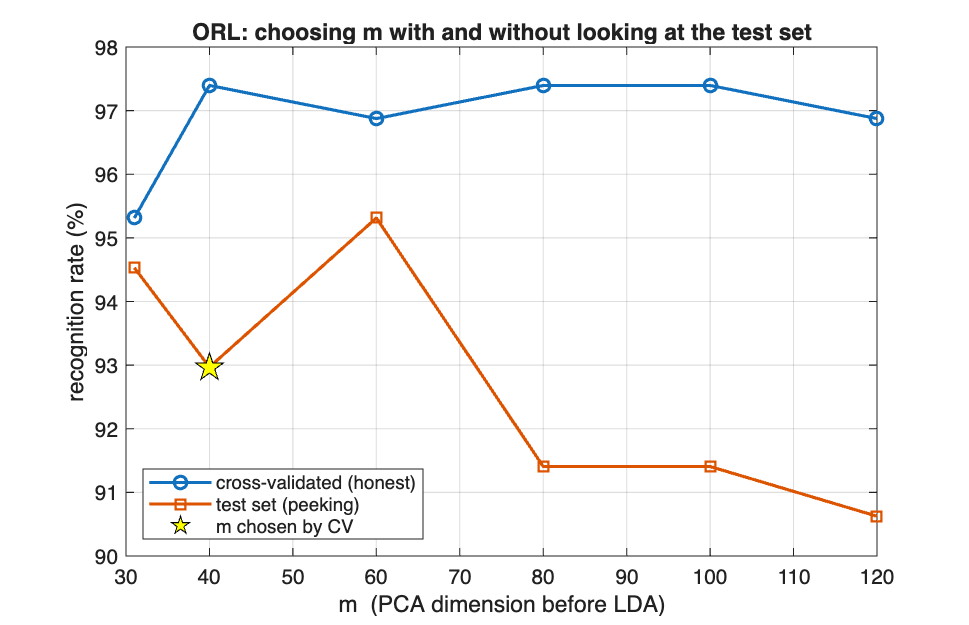
\includegraphics[width=0.68\textwidth]{figs_experiments/E3_cross_validation.png}
\caption{The honest curve and the peeking curve. The star marks the $m$ that
cross-validation selects, evaluated once on test.}
\end{figure}

\begin{observation}
\textbf{The $2.3$-point gap is the optimism we avoid by not peeking}, and it is
the single most useful number in this part. If asked ``is $95.3\%$ your real
accuracy?'', the correct answer is no: $95.3\%$ is what you get after letting
the test set choose a hyper-parameter, and the honest estimate is $93.0\%$.

Note also that the cross-validated rates ($\approx 97\%$) sit \emph{above} the
test rates. That is not a contradiction either: the validation images come from
the same six-image pool as the training images for that subject, which is an
easier problem than the held-out test images. Cross-validation is being used
here to \emph{rank} values of $m$, not to estimate the final accuracy.
\end{observation}

%% =====================================================================
\section{E4: a prediction, tested}

\paragraph{The question.} The frequency analysis measured Fisherfaces sitting
$3.85\times$ higher in spatial frequency than eigenfaces, because whitening
scales direction $l$ by $1/\sqrt{\lambda_l}$ and so amplifies the low-variance,
fine-detail directions most --- by up to $8860\times$ on ORL. White pixel noise
has energy at all frequencies. \textbf{Prediction: Fisherfaces should degrade
faster than eigenfaces as noise is added to the test images.}

This is the only experiment here that could have failed, which is what makes it
worth running.

\paragraph{The result, in two stages.} The first attempt swept
$\sigma \in \{0,5,10,20,40,80\}$ grey levels and found \emph{nothing}: all three
methods moved by $0.8$ points. On $128$ test images one image is worth
$100/128 = 0.78$ points, so ``$0.8$ points'' is \emph{one image} --- measurement
noise, not an effect.

The reason is that projection is a powerful denoiser. A unit-norm direction $v$
turns per-pixel noise of standard deviation $\sigma$ into coefficient noise of
standard deviation $\sigma$, because $\operatorname{Var}(v^{\!\top}n) = \sigma^2\|v\|^2 = \sigma^2$,
while the coefficients themselves are in the thousands. So $\sigma$ must become
very large before anything happens. Extending the sweep:

\begin{center}
\begin{tabular}{rccc}
\toprule
$\sigma$ & correlation & eigenfaces ($k=50$) & Fisherfaces \\
\midrule
  0 & $91.4\%$ & $95.3\%$ & $90.6\%$ \\
 20 & $92.2\%$ & $94.5\%$ & $89.8\%$ \\
 40 & $92.2\%$ & $94.5\%$ & $89.8\%$ \\
 80 & $93.0\%$ & $94.5\%$ & $89.1\%$ \\
160 & $89.1\%$ & $93.0\%$ & $81.2\%$ \\
320 & $85.2\%$ & $89.1\%$ & $60.9\%$ \\
640 & $58.6\%$ & $74.2\%$ & $30.5\%$ \\
\midrule
drop & $32.8$ pts & $\mathbf{21.1}$ pts & $\mathbf{60.2}$ pts \\
\bottomrule
\end{tabular}
\end{center}

\begin{figure}[htbp]
\centering
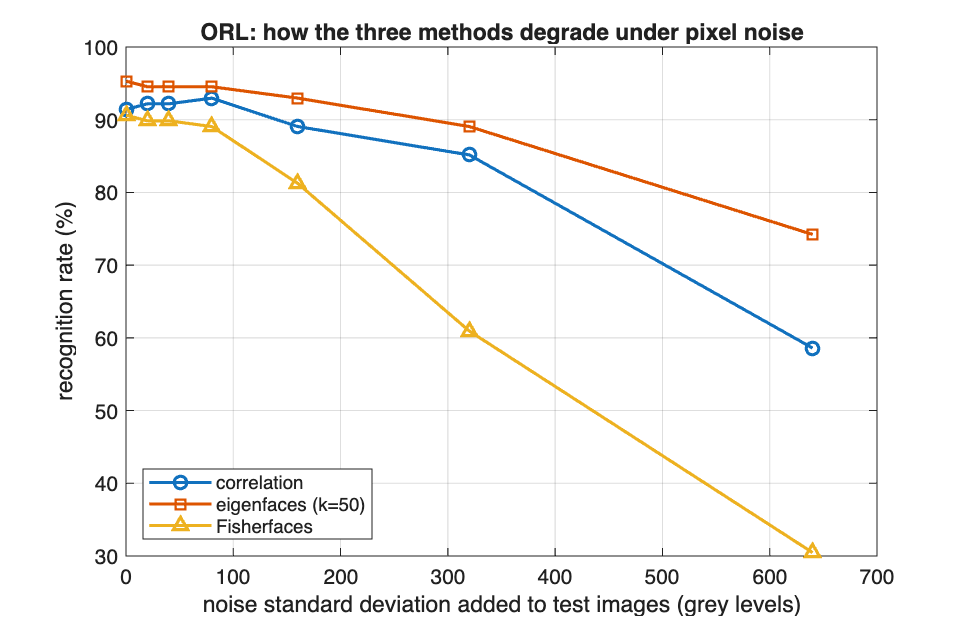
\includegraphics[width=0.68\textwidth]{figs_experiments/E4_noise.png}
\caption{Degradation under additive pixel noise. The curves are flat until
$\sigma \approx 80$ and then separate sharply.}
\end{figure}

\begin{observation}[Confirmed, with an honest caveat]
Fisherfaces lose $60.2$ points against eigenfaces' $21.1$, so the prediction
holds: the higher-frequency basis is roughly three times more fragile. But say
the caveat before he does --- \textbf{the effect only appears at noise levels far
beyond anything realistic.} Pixel values live on a $0$--$255$ scale, and nothing
measurable happens until $\sigma \approx 160$. At sensible noise levels the
three methods are indistinguishable, and reporting ``Fisherfaces are less
robust'' without that qualification would overstate the finding.
\end{observation}

%% =====================================================================
\section{E5: the paper's real protocol}

\paragraph{The question.} Our main table reports one Yale number per method.
The paper does not: it bins the test images by how far the light source is from
the camera axis and reports error per bin. That is far more informative,
because it shows \emph{where} each method fails.

\paragraph{The maths.} Every Yale filename encodes the light direction, e.g.
\texttt{yaleB01\_P00A+020E-40.pgm} means azimuth $+20^\circ$, elevation
$-40^\circ$. Treating azimuth and elevation as rotations about perpendicular
axes, the direction cosine along the camera axis is the product of the two
cosines, so the angle from the optical axis is
\[
  \theta \;=\; \arccos\big(\cos(\text{azimuth})\cdot\cos(\text{elevation})\big).
\]
The paper's five bins are $0$--$12^\circ$, $13$--$25^\circ$, $26$--$50^\circ$,
$51$--$77^\circ$ and above $77^\circ$.

\begin{lstlisting}
ia = strfind(nm, 'A');
ie = strfind(nm, 'E');
az = str2double(nm(ia+1 : ie-1));
el = str2double(nm(ie+1 : end-4));
theta(i) = acosd(cosd(az) * cosd(el));
\end{lstlisting}

\paragraph{The result.}

\begin{center}
\begin{tabular}{clrrr}
\toprule
subset & angle & images & eigenfaces error & Fisherfaces error \\
\midrule
1 & $0$--$12^\circ$   & \textbf{0}   & ---      & ---      \\
2 & $13$--$25^\circ$  & 104 & $1.0\%$  & $\mathbf{0.0\%}$ \\
3 & $26$--$50^\circ$  & 152 & $30.9\%$ & $\mathbf{2.0\%}$ \\
4 & $51$--$77^\circ$  & 300 & $88.3\%$ & $\mathbf{22.0\%}$ \\
5 & $>77^\circ$       & 338 & $93.8\%$ & $\mathbf{66.3\%}$ \\
\bottomrule
\end{tabular}
\end{center}

\begin{figure}[htbp]
\centering
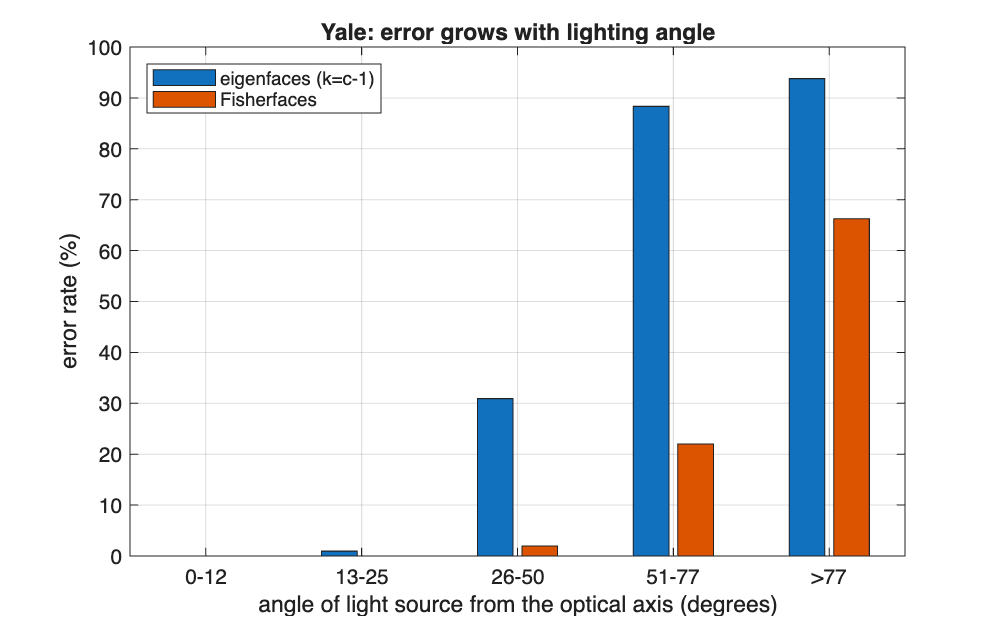
\includegraphics[width=0.72\textwidth]{figs_experiments/E5_illumination_subsets.png}
\caption{Error against lighting angle. Subset 1 is drawn as a gap rather than a
zero bar, because it contains no test images.}
\end{figure}

\begin{observation}[The paper's claim, at the resolution the paper makes it]
Error climbs with angle for both methods and the gap \emph{widens}: at
$26$--$50^\circ$ Fisherfaces are $15\times$ better ($2.0\%$ against $30.9\%$),
and even in the hardest bin they halve the error. This is the paper's central
claim --- that discarding within-class variation buys illumination robustness
--- measured where it actually bites, rather than averaged into a single
aggregate number.
\end{observation}

\begin{gotcha}[Subset 1 is empty, and that explains the headline numbers]
There are \textbf{no} test images at $0$--$12^\circ$. This is not a parsing bug;
it is the split bias of Section~\ref{sec:splitbias} reappearing. \texttt{dir}
sorts names as text and \texttt{'+'} sorts before \texttt{'-'}, so the first
$40$ files of each subject --- the training set --- absorb all the near-frontal
lighting. \emph{Every} test image is therefore at least $12^\circ$ off axis, and
most are far worse: $638$ of the $894$ test images sit beyond $50^\circ$.

That is the mechanism behind the poor headline Yale figures. The test set is
not a random sample of lighting conditions, it is the hard tail of one. Plotting
subset 1 as a zero bar would have read as a perfect score, which is why the
figure leaves a gap.
\end{gotcha}

%% =====================================================================
\section{What the five experiments add up to}

\begin{description}[leftmargin=*,style=nextline,nosep]
\item[The headline numbers are real.] E2: destroying the labels destroys the
  result, so nothing is leaking.
\item[But one of them was optimistic.] E3: $95.3\%$ became $93.0\%$ once $m$
  was chosen honestly. We report both and say which is which.
\item[The paper's $m = N-c$ is defensible but not optimal.] E1: better accuracy
  at smaller $m$ on both databases, and $\kappa(\Sw)$ smaller by five orders of
  magnitude there.
\item[The solver choice does not matter here, and we can prove it.] E1 again:
  Cholesky and the naive route agree to $0.00^\circ$ at every $m$ tested, while
  the round-off visibly grows with $\kappa$.
\item[One prediction survived testing, with a caveat.] E4: Fisherfaces really
  are more noise-fragile, but only far outside realistic noise levels.
\item[And the paper's claim is stronger than our summary table suggested.] E5:
  averaged over all lighting Fisherfaces win $67.2\%$ to $34.2\%$; split by
  angle they are $15\times$ better in the mid-range.
\end{description}
